\section{Graph in Data Engineering}
\subsection{Big Data lifecycle}
Il ciclo di vita dei sistemi che analizzano big data è composto da una serie di fasi:

\begin{itemize}
    \item \textbf{Collect}: i dati vengono raccolti da molteplici fonti.
    
    \item \textbf{Store}: i dati vengono memorizzati in modo adeguato in un unico (o talvolta più di uno) 
    archivio facilmente accessibile, per essere pronti alle fasi successive.
    
    \item \textbf{Clean}: i dati vengono unificati, puliti e, quando possibile, normalizzati usando uno 
    schema coerente e omogeneo.
    
    \item \textbf{Access}: i dati sono resi disponibili. Vengono fornite diverse viste o modalità di accesso 
    per semplificare e velocizzare l'accesso al dataset, che verrà poi utilizzato per l'addestramento.
\end{itemize}

\subsection*{Le 4 V dei Big Data}

Le principali caratteristiche che definiscono i Big Data sono riassunte nelle cosiddette \textbf{4 V}:

\begin{itemize}
    \item \textbf{Volume}: rappresenta la quantità enorme di dati generata ogni giorno da fonti diverse come social media, sensori, dispositivi mobili, log di sistema, ecc. La gestione richiede infrastrutture scalabili per l’archiviazione e l’elaborazione.

    \item \textbf{Velocità}: indica la rapidità con cui i dati vengono generati, trasmessi ed elaborati. In molti casi (es. mercati finanziari, IoT) è necessario un trattamento in tempo reale o quasi.

    \item \textbf{Varietà}: i dati provengono da fonti eterogenee e possono essere strutturati (es. tabelle), 
    semi-strutturati (es. JSON, XML) o non strutturati (es. testo libero, immagini, video, audio). L'integrazione e l'analisi di questi formati diversi è una sfida importante.

    \item \textbf{Veridicità}: si riferisce alla qualità, attendibilità e accuratezza dei dati. 
    I big data possono contenere rumore, dati mancanti o contraddittori; è quindi fondamentale valutare l’affidabilità delle fonti e pulire i dati prima dell’analisi.
\end{itemize}
\begin{figure}[th]
    \centering
    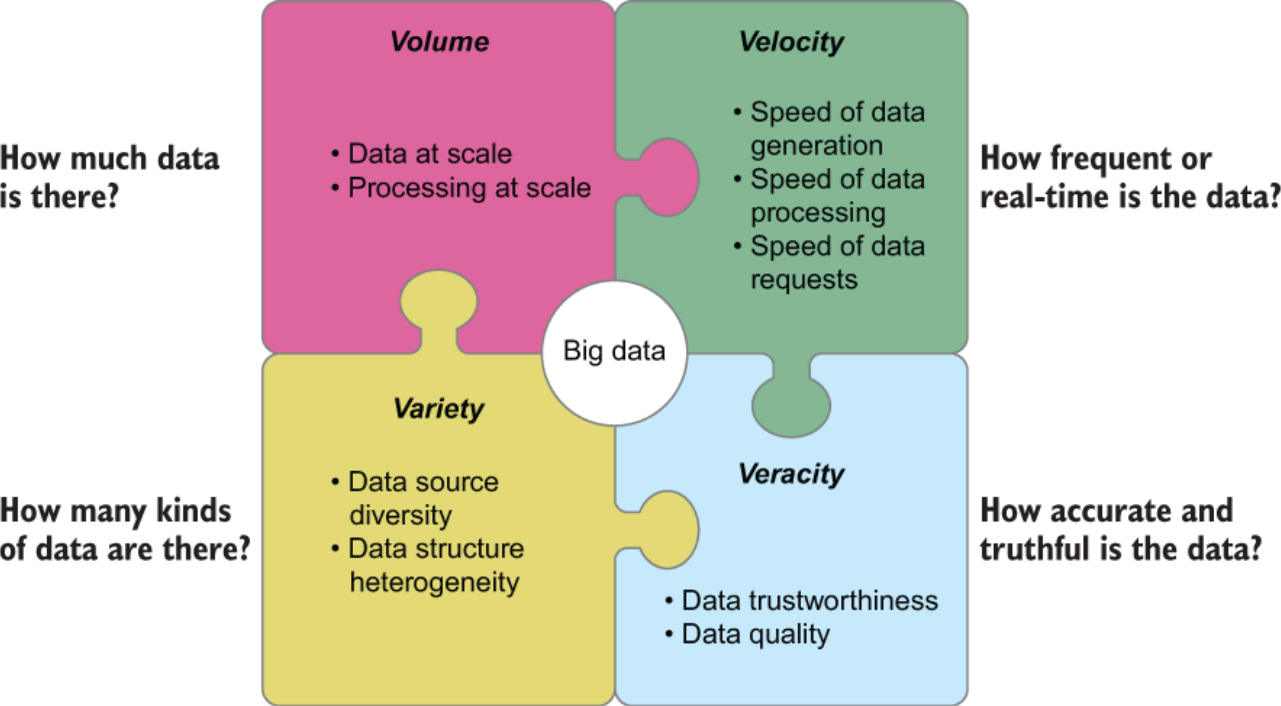
\includegraphics[width=0.65\linewidth]{GraphDataEngineering//img/4v.png}
\end{figure}

\paragraph{Use case scenario (slides)} Sei un poliziotto e vuoi tracciare un sospettato dalle chiamate telefoniche potendo monitorare i segnali del cellulare alle torri. Il nostro scopo in questo caso é quello di creare un modello predittivo sulla base dei dati di monitoring del telefono e prevedere le mosse a partire dalla location attuale. 
\\
\begin{figure}[th]
    \centering
    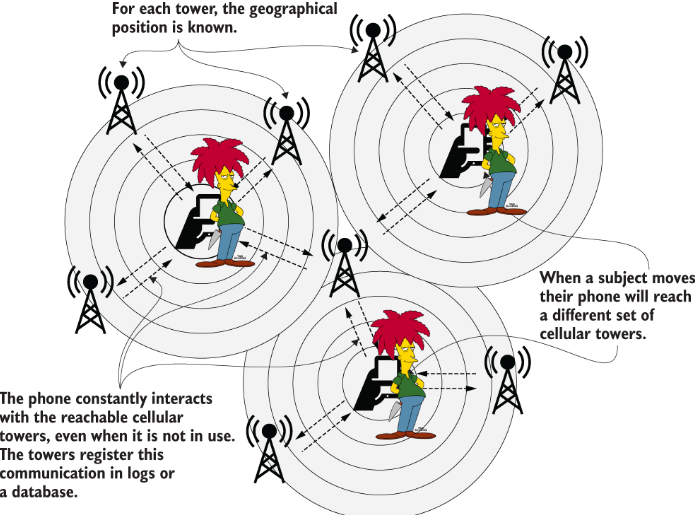
\includegraphics[width=0.5\linewidth]{ML&Graphs//img/esempiobob.png}
\end{figure}
\\
Per risolvere il problema possiamo fare uso dei grafi. Attraverso il loro utilizzo possiamo infatti generare i clusters che verranno successivamente analizzati da un modello. 
\\
\begin{figure}[th]
    \centering
    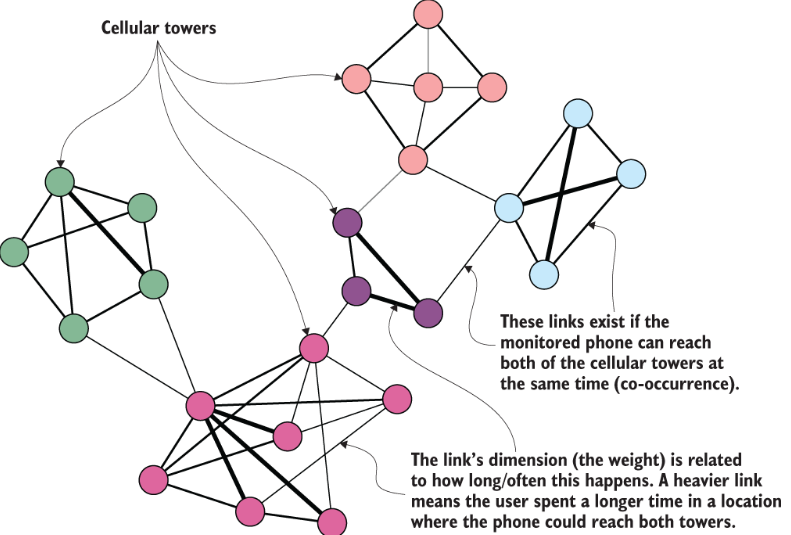
\includegraphics[width=0.5\linewidth]{GraphDataEngineering//img/esempioclusters.png}
\end{figure}
\\
Ognuno dei cellulari riesce a registrare le 4 torri piú vicine (quelle con il segnale piú forte). Una volta che vengono salvati questi dati possono essere rappresentati come CTN (cellular tower network) dove ogni nodo é una torre. I nodi sono presenti solo tra torri che compaiono contemporaneamente nello stesso record (quindi le 4 torri registrate dal singolo telefono saranno connesse) e ogni edge é pesato secondo una tempistica (quanto tempo la coppia é registrata insieme). \\
La \textbf{forza} di un nodo é misurata sulla somma dei pesi dei suoi edges. I nodi piú forti sono quelli piú vicini al cellulare. I cluster delle torri possono essere trasformati negli stati di un modello dinamico. Con i dati sugli spostamenti di un individuo, é infatti possibile prevedere con una buona precisione i suoi spostamenti futuri. Una volta che il modello sará allenato, si potrá prevedere a partire dalla posizione attuale la prossima location. 

\newpage

\paragraph{Architectural problems} Alcuni aspetti rilevanti di questo data flow, possono andare ad intaccare l'architettura del modello di ML:
\begin{itemize}
    \item \textbf{Eventi}: in questo caso i telefoni, quando mandano il segnale. Il signal non cambia e soprattutto avviene senza controllo. É importante fare lo storing dei dati una sola volta. 
    \item \textbf{Molteplici viste}: create come funzioni (ad esempio in questo caso aggregazione, clustering) ma possono cambiare in base all'algoritmo di learning. 
    \item \textbf{La creazione delle viste}: il processo normalmente lavora su tutti i dati disponibili, e puó richiedere del tempo. 
    \item \textbf{Real-time view}: avere una vista real-time si intende ovviamente \textbf{live}. É necessario un servizio streaming che legga gli eventi e registri nuovi dati subito.
\end{itemize}

\subsection{Lambda architecture}
Tutti questi problemi possono essere risolti utilizzando Lambda Architecture, che suddivide il problema big data in 3 parti: batch, serving e speed. 
\\
\begin{figure}[th]
    \centering
    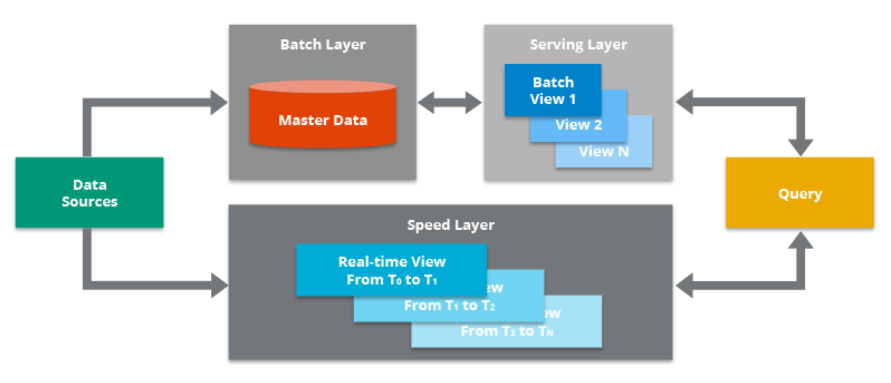
\includegraphics[width=0.6\linewidth]{GraphDataEngineering//img/lambdaarch.png}
\end{figure}
\\
Ogni layer si occupa di un subset di requisiti e lavora considerando le funzioni degli altri due. Contiene una pipeline batch ma anche una real-time per rispondere a richieste di ogni tipo. 
\subsubsection*{Layers di batch e di serving}
Tutti i dati nel formato raw sono salvati nel batch layer, oltre ad essere il responsabile dell'accesso a tali dati e al calcolo della batch view. Tutte le view risultanti sono salvate nel serving layer, dove sono indicizzate per essere piú accessibili. 
\\
\begin{figure}[th]
    \centering
    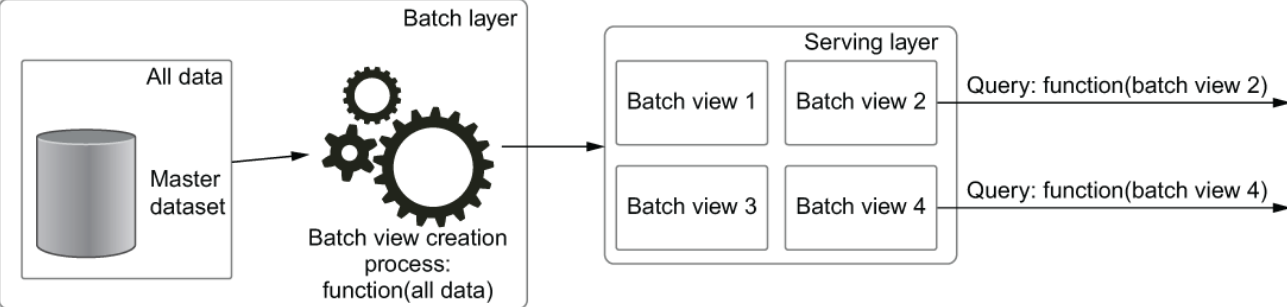
\includegraphics[width=0.7\linewidth]{GraphDataEngineering//img/batchserving.png}
\end{figure}
\\
Nello scenario CTN, con le torri e i segnali, una prima batch view sarebbe il grafo con le torri. La parte di creazione dei cluster viene fatta all'interno del batch layer e le nuove views vengono inviate al serving layer. 

\subsubsection*{Speed layer}
Lo speed layer fornisce delle view recenti, per coprire quel gap che c'é tra il batch layer e gli ultimi arrivati. Sfruttando sempre l'esempio del CTN:
\\
\begin{figure}[th]
    \centering
    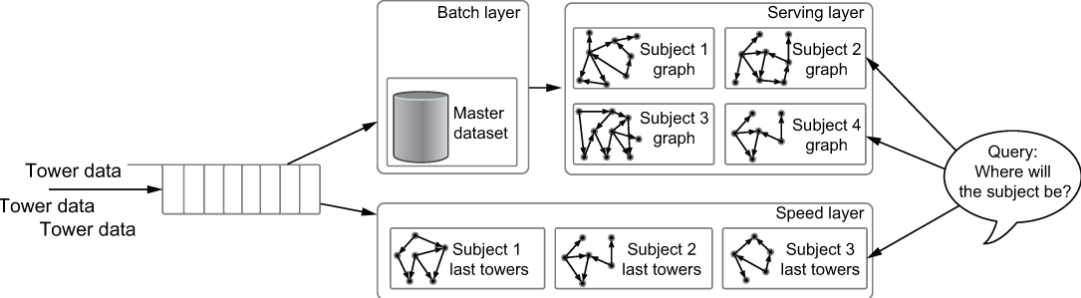
\includegraphics[width=0.8\linewidth]{GraphDataEngineering//img/speedlayer.png}
\end{figure}
\\
Nel CTN, sia la batch view che la real-time sono grafi. Questa rappresentazione non solo permette di rispondere piú velocemente a delle queries ma facilita ulteriormente l'analisi. La differenza sostanziale tra i due layer é che lo speed guarda solo gli ultimi arrivati. In questo scenario é lei che fornisce l'info sulla location attuale e su dove ci sposteremo. 

\paragraph{Conclusioni} Lambda architecture ha numerosi vantaggi architetturali che portano ad avere bassa latenza, buona data consistency, alta scalabilitá e una buona gestione di ogni tipo di errore. 

\subsection{Grafi per versioni fine-grained}
Esempio di fraud detection, vediamo gli approcci con graph: 

\subsubsection*{Primo Approccio - Grafi come Viste Aggregate}

I grafi vengono utilizzati per creare visualizzazioni sopra un dataset principale (\textit{batch layer}) o rappresentazioni in tempo reale (\textit{speed layer}) di porzioni dei dati disponibili. In questo caso, i dati transazionali risiedono altrove nel dataset principale, e questo approccio è utile quando si possono eseguire query e analisi su dati aggregati memorizzati nel \textit{serving layer}.

\subsubsection*{Secondo Approccio - Grafi come Fonte Principale}

Alcuni tipi di analisi non possono essere eseguite su versioni aggregate dei dati, ma richiedono algoritmi che necessitano di informazioni più dettagliate e granulari per essere efficaci. Anche in questo caso si può utilizzare il modello a grafo per rappresentare le connessioni e sfruttare gli \textit{insight} dai dati.

\subsubsection*{Vantaggio Chiave}

Comprendere le connessioni tra i dati e derivare significato da questi collegamenti offre capacità che non sono disponibili nei metodi analitici classici non basati sui grafi. In quest'ultimo caso, il grafo diventa la fonte principale di conoscenza e modella un'unica fonte di verità connessa.

\vspace{0.5cm}

\noindent \textbf{Conclusione:} In sostanza, il testo contrappone l'uso dei grafi come strumento di visualizzazione versus il loro utilizzo come struttura dati fondamentale per l'analisi.

\newpage
\subsection{Vantaggi dei grafi}
Vediamo i vantaggi dei grafi nell'analisi dei dati nel dettaglio:
\begin{itemize}
    \item \textbf{Integrazione di Fonti Multiple:} Diverse fonti di dati, come informazioni geografiche o GPS, dati dei social network, profili personali degli utenti, dati familiari e simili, possono essere unite in un'unica fonte di verità connessa.
    
    \item \textbf{Estensione con Fonti Esterne:} I dati esistenti possono essere arricchiti con fonti esterne di conoscenza (posizioni dei negozi, indirizzi delle persone, ecc.) o con informazioni contestuali (un nuovo negozio, altri reclami, ecc.) che possono essere utilizzate per migliorare l'analisi.
    
    \item \textbf{Supporto a Tecniche Multiple:} Lo stesso modello dati può supportare diverse tecniche di analisi. Ad esempio, per scoprire un \textit{fraud ring} -- "un'organizzazione focalizzata sulla truffa delle persone. Falsificazioni, false dichiarazioni, furto d'identità, contraffazione di assegni e valute sono tutte attività fraudolente."
    
    \item \textbf{Visualizzazione e Analisi Manuale:} I dati possono essere visualizzati come grafo per accelerare l'analisi manuale. L'analisi può essere estesa a molteplici livelli di interazione, considerando salti multipli (\textit{multiple hops}).
    
    \item \textbf{Semplificazione delle Operazioni:} La struttura semplifica le operazioni di fusione e pulizia dei dati, grazie al pattern di accesso flessibile fornito dal modello a grafo.
\end{itemize}

\subsection{Grafi come Master Data Management (MDM)}
Con master data management si intende il ruolo che hanno i grafi nella gestione dei dati: la capacitá di identificare, fare cleaning, salvare e controllare i dati. Questo perché si evolvono con il tempo, aggiungo nuove fonti di dati, aggiornano i dati attuali sulla base di fonti esterne, e fare data versioning per gestire al meglio i dati obsoleti. 
\\
Simili a DataWarehouses ma diversi. I graph based MDM hanno i seguenti vantaggi:
\begin{itemize}
    \item \textbf{Flessibilità:} I dati acquisiti possono essere facilmente modificati per includere attributi e oggetti aggiuntivi.
    
    \item \textbf{Estensibilità:} Il modello consente la rapida evoluzione del modello di dati master in linea con le esigenze aziendali in evoluzione.
    
    \item \textbf{Capacità di Ricerca:} Ogni nodo, ogni relazione e tutte le loro proprietà correlate sono punti di accesso per la ricerca.
    
    \item \textbf{Capacità di Indicizzazione:} I database a grafo sono naturalmente indicizzati sia per relazioni che per nodi, fornendo un accesso più veloce rispetto ai dati relazionali.
\end{itemize}

In un progetto ML é necessario seguire diversi step per l'utilizzo dei grafi: ovvero come si fa modeling (come rappresentare i dati usando il grafo) come gestire lo storage (serve avere uno storage dei dati persistent, in modo da poter sempre accedere ai dati)  e piú importante, gestire la fase di processing dei dati. Quando si lavora con grandi quantitativi di dati inoltre é difficile gestirli contemporaneamente quindi su opta per tecniche di \textbf{sharding} dove i grandi set vengono suddivisi in shards. Ma con i grafi non é cosí semplice: una possibile soluzione é quella di mettere tutti i nodi connessi all'interno dello stesso shard, per ridurre la latenza nel caso di navigazione del grafo; questo comunque comporta grandi costi nel traversare il grafo soprattutto quando si cerca un'informazione in uno shard separato che comunque é connessa ad un nodo dello shard attuale (basta pensare alla struttura a di un grafo connesso e due nodi distanti ma connnessi). 

\subsubsection*{Tecniche per lo sharding coi grafi}
Esistono tre tecniche principali per gestire lo sharding che sono:
\begin{itemize}
    \item Application Level Sharding: come indica il nome, viene tutto lasciato in mano all'applicazione che suddivide nel modo che piú aggrada. 
    \item Utilizzo di cache sharding o aumento della memoria: aumentare la memoria puó garantire che tutto il grafo stia in memoria. Cache sharding i dati vengono distribuiti su multiple istanze di cache (shard) utilizzando una funzione di hash o altri algoritmi di partizionamento.
\end{itemize}

\subsubsection*{Tecniche di replication}
In particolare, parlando di replication, il problema si presenta piú complesso del previsto, perché entra in gioco anche la gestione delle repliche: una decisione fondamentale quando si fa sincronizzazione é scegliere quale delle parti viene aggiornata per prima; si parla di di:
\begin{itemize}
    \item \textbf{Sistema centralizzato}: quando i primi updates sono fatti su una master copy, quelle che gestiscono tutte le operazioni.
    \item \textbf{Sistema distribuito}: quando i primi updates sono sulle repliche direttamente.
\end{itemize}
La differenza tra master e replica nella replication é semplicemente che come in ogni altro sistema di replication, il master é il primo nodo ad essere aggiornato e ha il compito di diffondere l'aggiornamento a tutte le sue repliche. 

\subsubsection*{Native e non-native graph databases}
Ci sono numerosi metodi per rappresentare grafi all'interno di un database. \textbf{Native graph databases} sono progettati per creare un filesystem che supporti in ogni modo il grafo oltre a comprenderlo, rendendoli altamente performanti. Per essere piú precisi, ogni nodo mantiene un riferimento diretto ai suoi nodi adiacenti (\textbf{index free adjacency}).

\paragraph{Non native graph dbms} Consiste in un dbms specializzato in un altro tipo di dato (colonne, relazionale, ecc...) quindi quando deve lavorare con dei grafi c'é sempre da fare anche una conversione dei dati in ingresso. Quindi un non native sará sempre meno performante del native, appunto per questa caratteristica. Esistono due tipi di non native: quelli che inseriscono un layer graph API a monte di una struttura dati giá esistente e quelli che integrano piú strutture dati in una con semantica multimodello.

\paragraph{Vantaggi dei modelli native} Vediamo i pro:
\begin{itemize}
  \item \textbf{Prestazioni “da minuti a millisecondi”}: I database a grafo nativi gestiscono le query su dati connessi molto più velocemente rispetto ai database non nativi. Anche su hardware modesto, i database a grafo nativi possono facilmente gestire milioni di attraversamenti al secondo tra nodi su una singola macchina e molte migliaia di scritture transazionali al secondo.
  
  \item \textbf{Efficienza in lettura}: I database a grafo nativi offrono attraversamenti a tempo costante grazie all’adiacenza senza indice, senza la necessità di progettazioni complesse dello schema o ottimizzazioni delle query. Il modello intuitivo dei grafi a proprietà elimina la necessità di logiche applicative aggiuntive e spesso complesse per elaborare le connessioni.
  
  \item \textbf{Ottimizzazione dello spazio su disco}: Per migliorare le prestazioni in un grafo non nativo, è possibile denormalizzare gli indici o crearne di nuovi, o entrambe le cose, il che incide sulla quantità di spazio necessaria per memorizzare le stesse informazioni.
  
  \item \textbf{Efficienza in scrittura}: La denormalizzazione degli indici ha un impatto anche sulle prestazioni in scrittura, poiché tutte le strutture di indice aggiuntive devono essere aggiornate anch’esse.
\end{itemize}

\subsubsection*{Label Property Graphs (LPG)}
Altro metodo per la gestione big data nel caso di Graph Database Management. Modello per la struttura a grafo dove vengono labellati nodi e archi. Con questo modello é possibile sfruttare operazioni normalmente attribuibili ad altri DBMS, come proiezione, selezione, grouping, filtering...
\\
Secondo il progetto openCypher, un \textit{label property graph} è definito come “un multigrafo diretto, con vertici etichettati, archi etichettati, archi che possono essere auto-collegamenti, in cui gli archi hanno una propria identità.” Un'\textbf{etichetta} è una stringa di testo che identifica un tipo, un insieme o una categoria di dati o oggetti. Nel mondo dei grafi, un'etichetta identifica un nodo o una relazione (vertice o arco).
\begin{itemize}
    \item Un oggetto etichettato in un grafo è opzionale e non deve necessariamente essere unico.
    \item Un oggetto etichettato è simile a un tag che indica un certo tipo di raggruppamento o categoria.
    \item È possibile applicare più etichette a un oggetto nel grafo.
\end{itemize}

\begin{figure}[th]
    \centering
    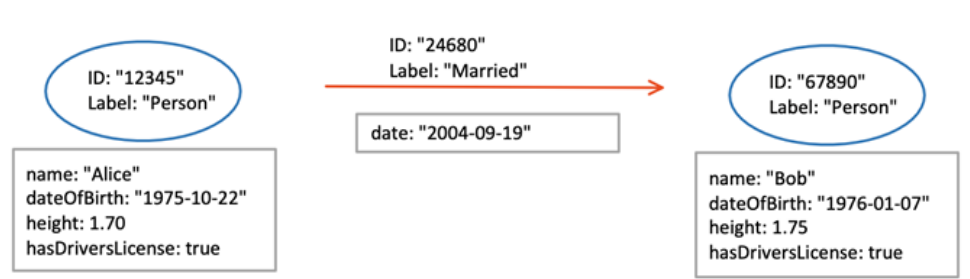
\includegraphics[width=0.65\linewidth]{GraphDataEngineering//img/lpg.png}
\end{figure}

\subsubsection*{Proprietà di un Label Property Graph (LPG)}

Un \textit{Label Property Graph} possiede le seguenti proprietà (definite in modo indipendente dalla piattaforma):

\begin{itemize}
  \item Il grafo è costituito da un insieme di entità. Un'entità rappresenta un nodo oppure una relazione.
  
  \item Ogni entità ha un identificatore che la identifica univocamente all'interno dell'intero grafo.
  
  \item Ogni relazione ha una direzione, un nome che ne identifica il tipo, un nodo di partenza e un nodo di arrivo.
  
  \item Un'entità può avere un insieme di proprietà, solitamente rappresentate come coppie chiave/valore.
  
  \item I nodi possono essere etichettati con una o più etichette, che li raggruppano e indicano i ruoli che essi svolgono all'interno del dataset.
\end{itemize}